\documentclass[tikz,border=0pt]{standalone}
\usepackage{amsmath,amssymb}
% Times text (Nimbus, as imsart loads it) with Computer Modern math, as in the paper
\usepackage[T1]{fontenc}
\usepackage{times}
\usetikzlibrary{arrows.meta,calc}
\definecolor{directed}{HTML}{1B4F72}
\definecolor{bidirected}{HTML}{E67E22}
\definecolor{ink}{HTML}{1F1F1F}
\definecolor{mid}{HTML}{6B6B6B}
\definecolor{rule}{HTML}{A6A6A6}
\definecolor{stagefill}{HTML}{EDF2F6}
\definecolor{sidefill}{HTML}{F4F4F4}
\newcommand{\Emin}{\mathcal E_{\min}}
\newcommand{\K}{\mathcal K}
% assumption chip: orange letter in a thin rounded box
\newcommand{\as}[1]{\tikz[baseline=(t.base)]\node[draw=bidirected,
  line width=.5pt,rounded corners=1.2pt,inner xsep=1.5pt,inner ysep=.8pt,
  text=bidirected,font=\bfseries\fontsize{7.5}{8}\selectfont] (t) {#1};}
\newcommand{\scope}[1]{\,{\color{mid}#1}}
\newcommand{\res}[1]{{\bfseries\color{directed}#1}}
\newcommand{\verdict}[1]{{\bfseries\color{directed}#1}}
\newcommand{\stagehead}[2]{{\bfseries #1}\ {\itshape #2}\par\vspace{1pt}}
% results line of a stage: result numbers, section in gray, assumption chips
\newcommand{\resline}[3]{\par\vspace{2pt}\res{#1}\quad{\color{mid}#2}\hfill#3}
\begin{document}
\hyphenpenalty=10000 \exhyphenpenalty=10000
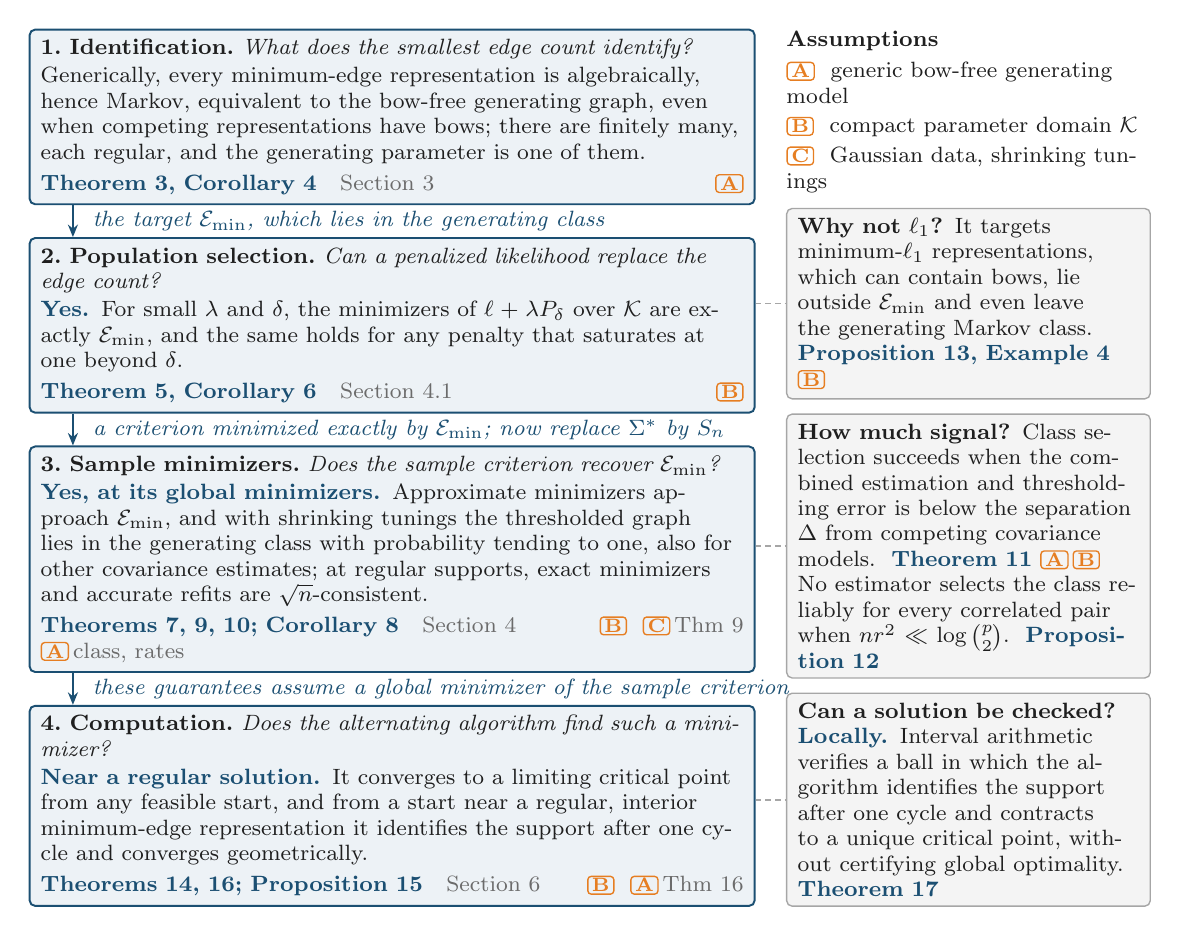
\begin{tikzpicture}[x=1pt,y=1pt,color=ink,
  stage/.style={draw=directed,line width=.7pt,fill=stagefill,
    rounded corners=2pt,anchor=north west,text width=254pt,align=left,
    inner xsep=4pt,inner ysep=3.5pt,
    font=\fontsize{8}{9.2}\selectfont},
  side/.style={draw=rule,line width=.5pt,fill=sidefill,rounded corners=2pt,
    text width=123.4pt,align=left,inner xsep=4pt,
    inner ysep=3.5pt,
    font=\fontsize{8}{9.2}\selectfont},
  arrow/.style={-{Stealth[length=4.5pt,width=3.6pt]},draw=directed,
    line width=.8pt},
  hlabel/.style={anchor=west,inner sep=0pt,
    font=\itshape\fontsize{8}{9}\selectfont,text=directed},
  link/.style={draw=rule,line width=.6pt,dash pattern=on 2pt off 1.5pt}]

\def\gap{11.5}   % vertical gap between stages; it holds the arrow label
\def\xside{274}

% stages ---------------------------------------------------------------------
\node[stage] (S1) at (0.35,-0.35) {%
  \stagehead{1.\ Identification.}{What does the smallest edge count identify?}
  Generically, every minimum-edge representation is algebraically, hence
  Markov, equivalent to the bow-free generating graph, even when competing
  representations have bows; there are finitely many, each regular, and
  the generating parameter is one of them.
  \resline{Theorem 3, Corollary 4}{Section 3}{\as{A}}};

\node[stage] (S2) at ($(S1.south west)+(0,-\gap)$) {%
  \stagehead{2.\ Population selection.}{Can a penalized likelihood replace the edge count?}
  \verdict{Yes.} For small $\lambda$ and $\delta$, the minimizers of
  $\ell+\lambda P_\delta$ over $\K$ are exactly $\Emin$, and the same holds
  for any penalty that saturates at one beyond $\delta$.
  \resline{Theorem 5, Corollary 6}{Section 4.1}{\as{B}}};

\node[stage] (S3) at ($(S2.south west)+(0,-\gap)$) {%
  \stagehead{3.\ Sample minimizers.}{Does the sample criterion recover $\Emin$?}
  \verdict{Yes, at its global minimizers.} Approximate minimizers approach
  $\Emin$, and with shrinking tunings the thresholded graph lies in the
  generating class with probability tending to one, also for other
  covariance estimates; at regular supports, exact minimizers and accurate
  refits are $\sqrt n$-consistent.
  \resline{Theorems 7, 9, 10; Corollary 8}{Section 4}%
    {\as{B}\ \ \as{C}\scope{Thm 9}\ \ \as{A}\scope{class, rates}}};

\node[stage] (S4) at ($(S3.south west)+(0,-\gap)$) {%
  \stagehead{4.\ Computation.}{Does the alternating algorithm find such a minimizer?}
  \verdict{Near a regular solution.} It converges to a limiting critical
  point from any feasible start, and from a start near a regular, interior
  minimum-edge representation it identifies the support after one cycle
  and converges geometrically.
  \resline{Theorems 14, 16; Proposition 15}{Section 6}{\as{B}\ \ \as{A}\scope{Thm 16}}};

% arrows between stages ---------------------------------------------------------
\foreach \a/\b/\lab in {
  1/2/{the target $\Emin$, which lies in the generating class},
  2/3/{a criterion minimized exactly by $\Emin$; now replace $\Sigma^*$ by $S_n$},
  3/4/{these guarantees assume a global minimizer of the sample criterion}}{
  \draw[arrow] ($(S\a.south west)+(16,0)$) -- ($(S\b.north west)+(16,0)$);
  \node[hlabel] at ($(S\a.south west)!.5!(S\b.north west)+(23,0)$) {\lab};
}

% side column ------------------------------------------------------------------
\node[anchor=north west,inner sep=0pt,text width=131.4pt,align=left,
      font=\fontsize{8}{9.2}\selectfont] (K) at (\xside,-1.2) {%
  {\bfseries Assumptions}\par\vspace{2pt}
  \as{A}\ \ generic bow-free generating model\par\vspace{1.5pt}
  \as{B}\ \ compact parameter domain $\K$\par\vspace{1.5pt}
  \as{C}\ \ Gaussian data, shrinking tunings};

\node[side,anchor=south west] (T4) at ($(S4.south west)+(\xside-0.35,0)$) {%
  {\bfseries Can a solution be checked?} \verdict{Locally.} Interval
  arithmetic verifies a ball in which the algorithm identifies the support
  after one cycle and contracts to a unique critical point, without
  certifying global optimality.\ \ \res{Theorem 17}};

\node[side,anchor=south west] (T3) at ($(T4.north west)+(0,5)$) {%
  {\bfseries How much signal?} Class selection succeeds when the combined
  estimation and thresholding error is below the separation $\Delta$ from
  competing covariance models.\ \ \res{Theorem 11}\ \as{A}\,\as{B}\ \ No
  estimator selects the class reliably for every correlated pair when
  $nr^2\ll\log\binom p2$.\ \ \res{Proposition 12}};

\node[side,anchor=south west] (T2) at ($(T3.north west)+(0,5)$) {%
  {\bfseries Why not $\ell_1$?} It targets minimum-$\ell_1$
  representations, which can contain bows, lie outside $\Emin$ and even
  leave the generating Markov class.\ \ \res{Proposition 13,
  Example 4}\ \as{B}};

\foreach \i in {2,3,4}{
  \draw[link] (S\i.east |- T\i.west) -- (T\i.west);
}
\path (S4.south); \pgfgetlastxy{\xb}{\yb}\pgfmathsetmacro{\ybot}{-\yb+0.35}
\pgfresetboundingbox
\path[use as bounding box] (0,0) rectangle (406,{-\ybot});
\end{tikzpicture}
\end{document}
